
Duplicate content\textemdash{}memory pages and disk blocks\textemdash{}is a common
occurence in virtualization-based hosting of applications, where
virtual machines (VMs) are instantiated from the same image 
template~\cite{effectiveness} or execute similar software environments. 
A study of content similarity amongst 525
virtual images from a production remote desktop environment~\cite{similarity}, 
reported that
30\% blocks were found to repeat at least twice and 12\% blocks were
found to repeat 5 times. A follow-up study\cite{vdn}
reported median of pairwise similarity across
virtual machine images to be around 48\%.

Content similarity within a single virtual machine image is referred
as \textit{intra-VM} similarity, whereas across multiple images, it is
referred as \textit{inter-VM} similarity.
A study in \cite{intra-higherthan-inter} has reported that, in general,
intra-VM similarity is significant, with up to 90\% of total similarity 
observed among VM disk content being intra-VM.
The work in \cite{iodedup} studied the degree of content similarity
in application workloads (web, mail and file system) hosted in 
individual virtual machines,
and reported that the amount of unique content accessed is lesser
than the unique number of blocks accessed, implying that there are multiple 
blocks having identical content within each application workload.

\begin{figure}[t]
\centering
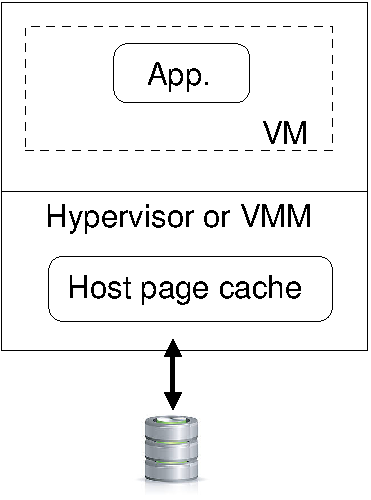
\includegraphics[scale=0.65]{confided-figures/main/system-under-considerat.pdf}
\vspace{-0.15in}
\caption{Typical Virtualized System Under Consideration}
\label{fig:system-under-considerat}
%%\vspace{-0.2in}
\end{figure}

Consider the system illustrated in Fig.\ref{fig:system-under-considerat}.
When an application or service (example, mail server or web server) is deployed 
within a VM instantiated on a host,
the virtual disk corresponding to the VM is present on the host's storage.
The storage may be a \textit{local} disk or a network-attached
\textit{remote} disk.
As discussed above, virtualized systems have inherent content similarity
among the data content that resides on disk, and this data is fetched 
from disk by corresponding applications. 
Disk access times are usually in the order of a few 
milliseconds\cite{google, data-domain}, whereas in comparison, 
host cache access timings are orders of magnitudes lower\cite{pagecache}. 
Hence, improving caching
effectiveness can, in general, help improve storage access performance
and overall application performance.


Harnessing content similarity 
to avoid duplicate disk I/O requests %that fetch the same content
is referred as I/O deduplication.
To harness content similarity across different blocks,~\cite{iodedup} 
suggests the use of a 
\textit{content-based cache} which can be looked up by content also.
Work in \cite{iodedup} demonstrates that a 
given limited size cache can be better utilized if used based on
content, rather than blocks.
However, by introducing a new content-cache, it introduces
cache inclusiveness concerns among the two caches. Also, the
split-cache design of reserving a part of existing block-cache as
a content-cache implies that content-cache performance is
achieved at the cost of precious block-cache space, as studied later
in this chapter.
